% !Mode:: "TeX:UTF-8:Main"

\documentclass{article}
\usepackage{l3pdf}
\usepackage{pdfresources}
\ExplSyntaxOn
\pdf_uncompress:
\ExplSyntaxOff

\usepackage{ifluatex,graphicx}
\usepackage{pdfpages,xcolor}
\usepackage[customdriver=hgeneric-experimental]{hyperref}
\hypersetup{linkbordercolor=red}
\hypupdateattribute

\ifluatex
\directlua{
 require("newpax")
 newpax.writenewpax("pax-input")
 %newpax.writepax("pax-input")
 newpax.writenewpax("figure/pax-input2")
% newpax.writenewpax("example-image-a")
 %newpax.writenewpax("C:/texlive/2020/texmf-dist/doc/latex/biblatex/biblatex")
 %newpax.writenewpax("C:/texlive/2020/texmf-dist/doc/latex/pgfplots/pgfplots")
 }
\fi

\usepackage{newpax}

\newpaxsetup{usefileattributes}


\begin{document}\raggedright
%\includepdf[pages=-]{C:/texlive/2020/texmf-dist/doc/latex/pgfplots/pgfplots}
included graphic:
%\tracingmacros=1
\fbox{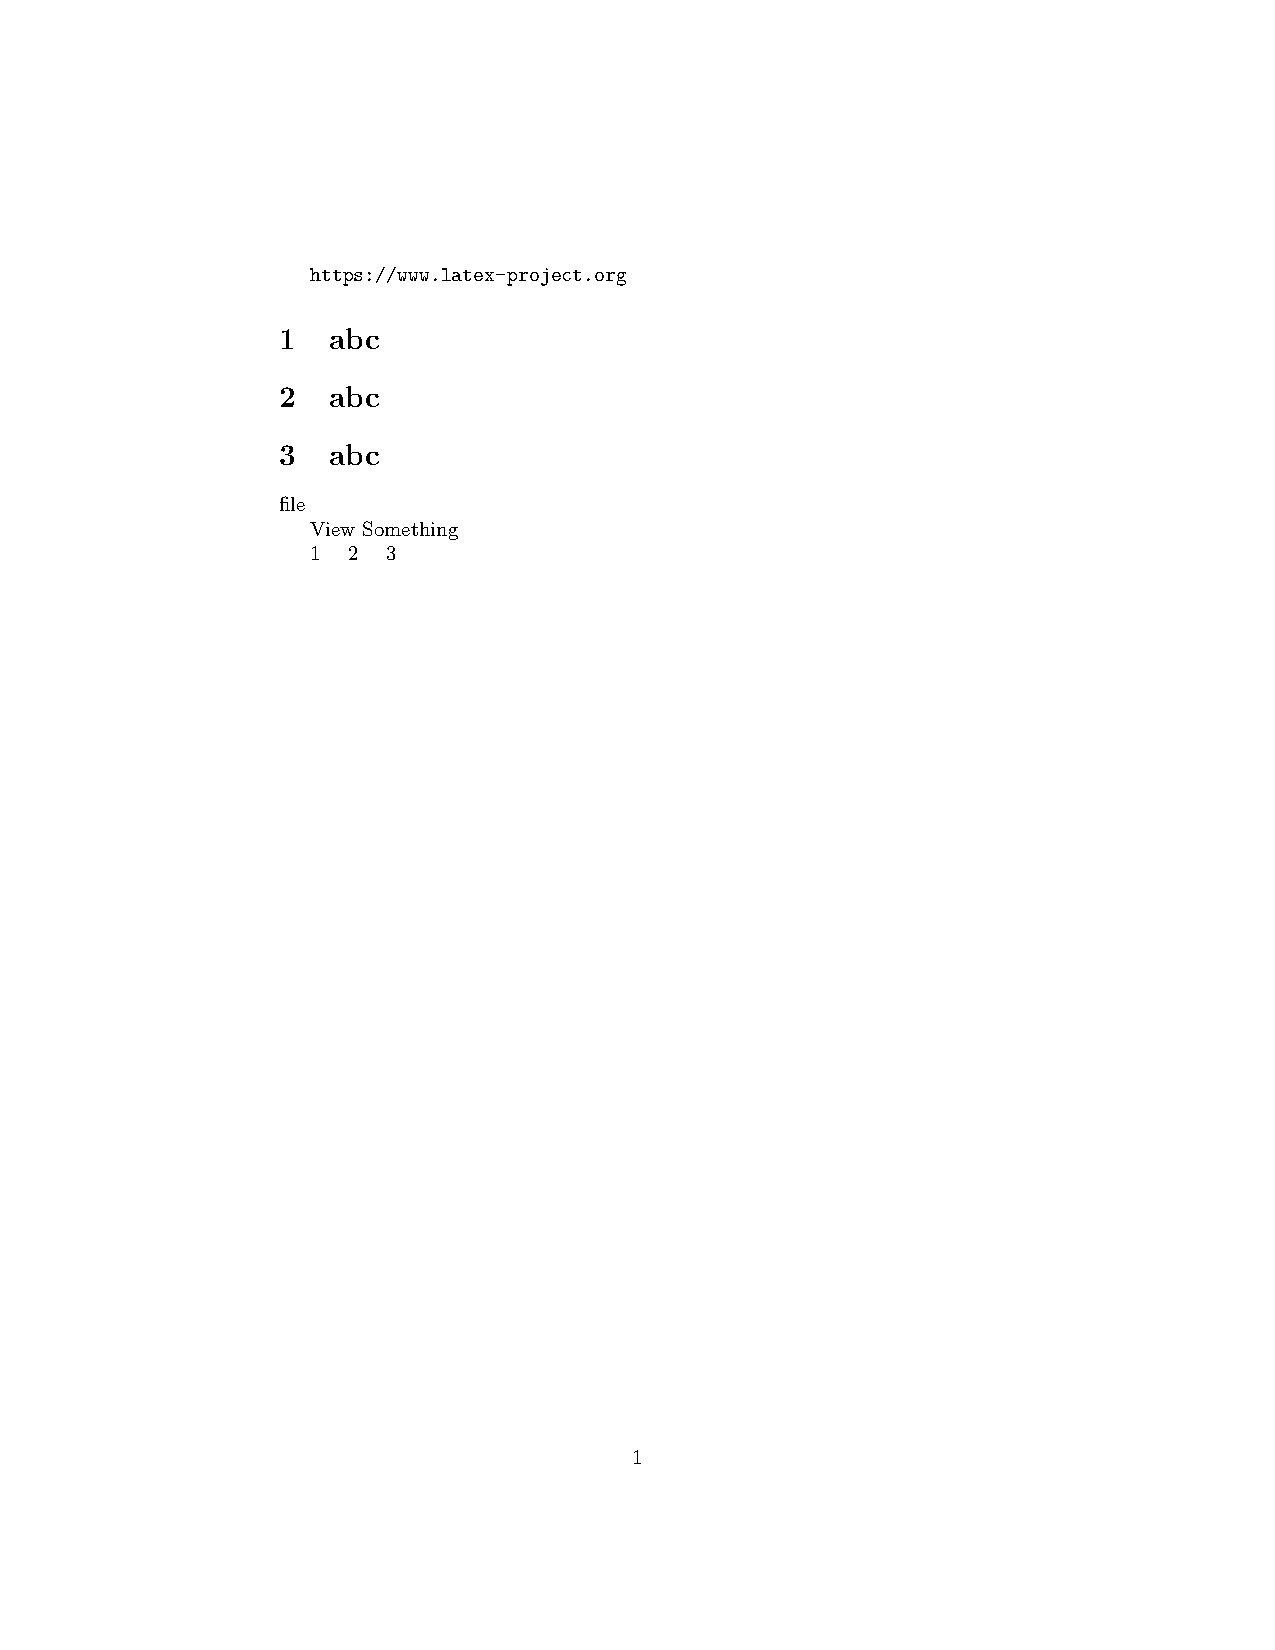
\includegraphics{pax-input}}
\fbox{\includegraphics[page=2]{pax-input}}

%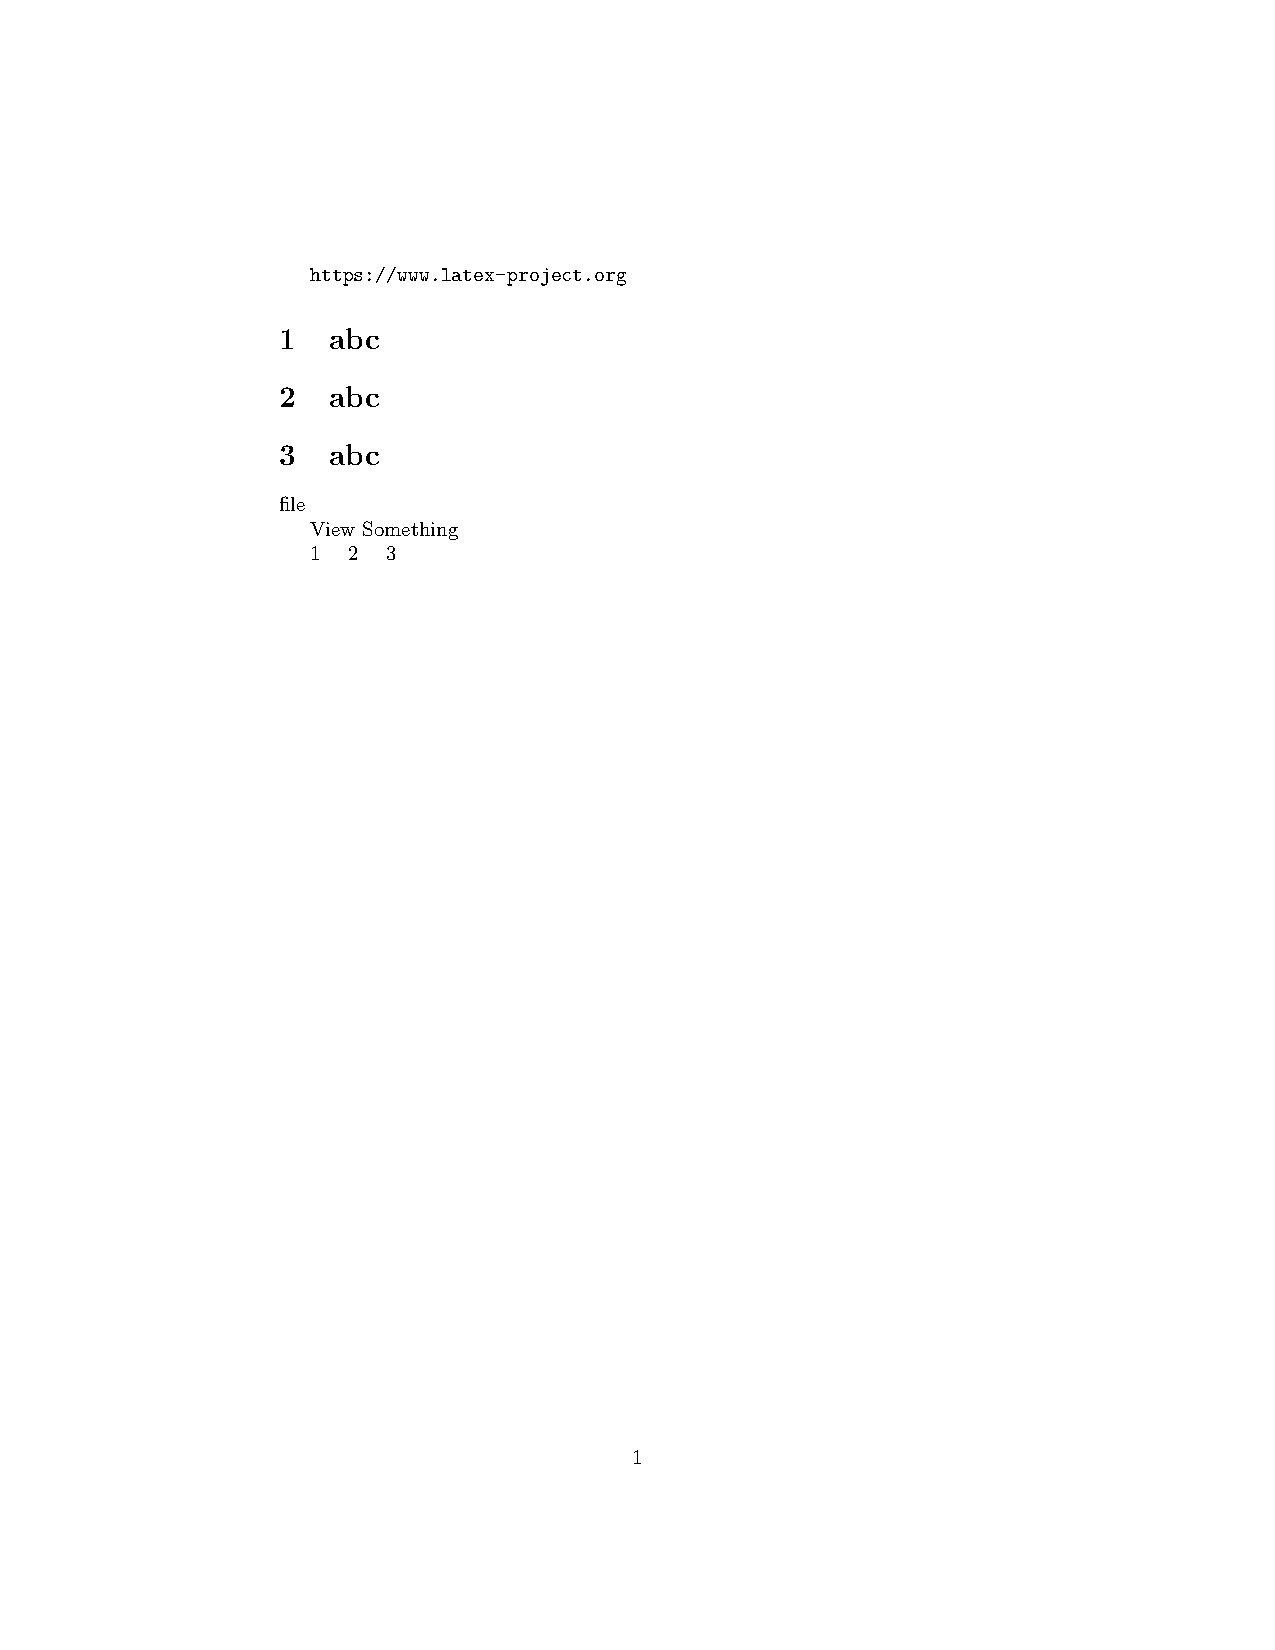
\includepdf{pax-input}
\end{document}
\fbox{\includegraphics[scale=0.5,trim=5cm 15cm 8cm 3cm,clip,page=2]{pax-input}}

%\newpaxsetup{useattributes=false,destsuffix=B}

%\newpaxsetup{addannots=false}
\fbox{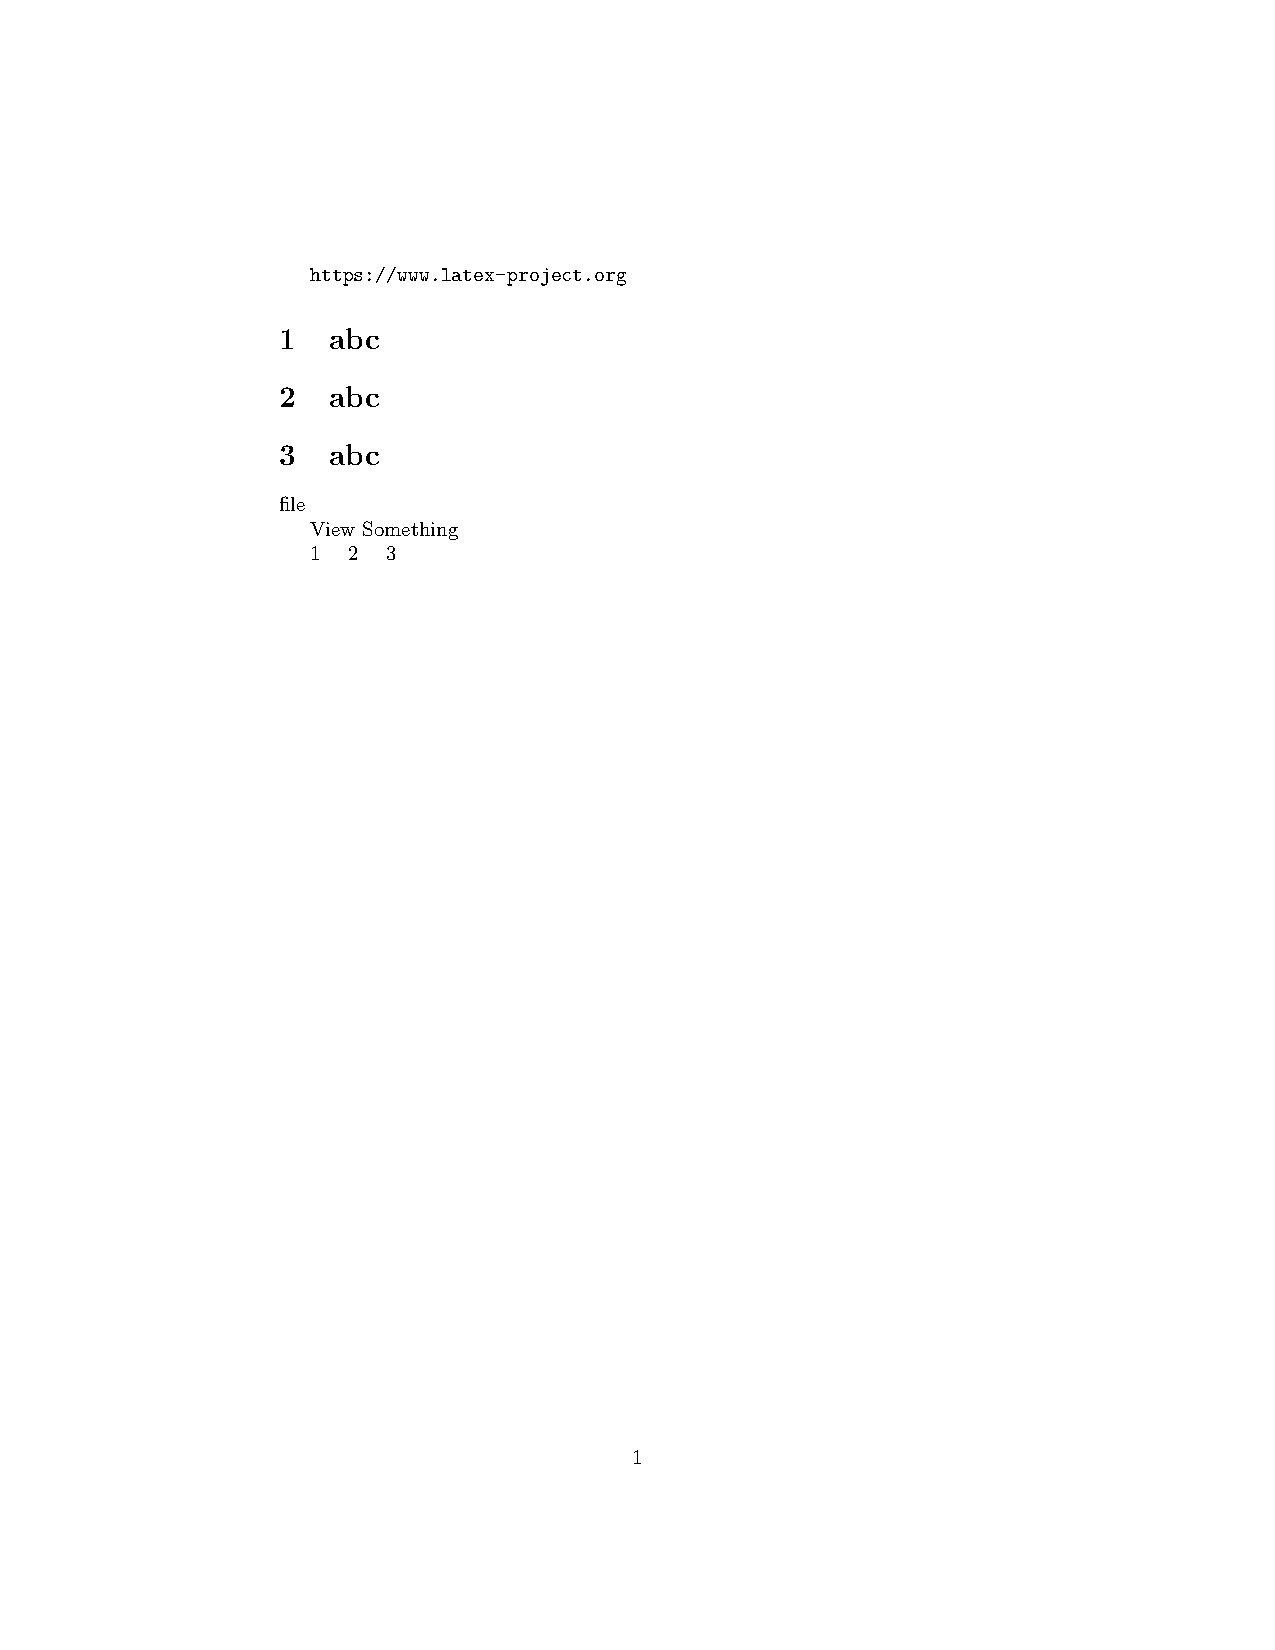
\includegraphics[scale=0.5,trim=4cm 15cm 8cm 3cm,clip,page=1]{pax-input}}

%\newpaxsetup{addannots=true}
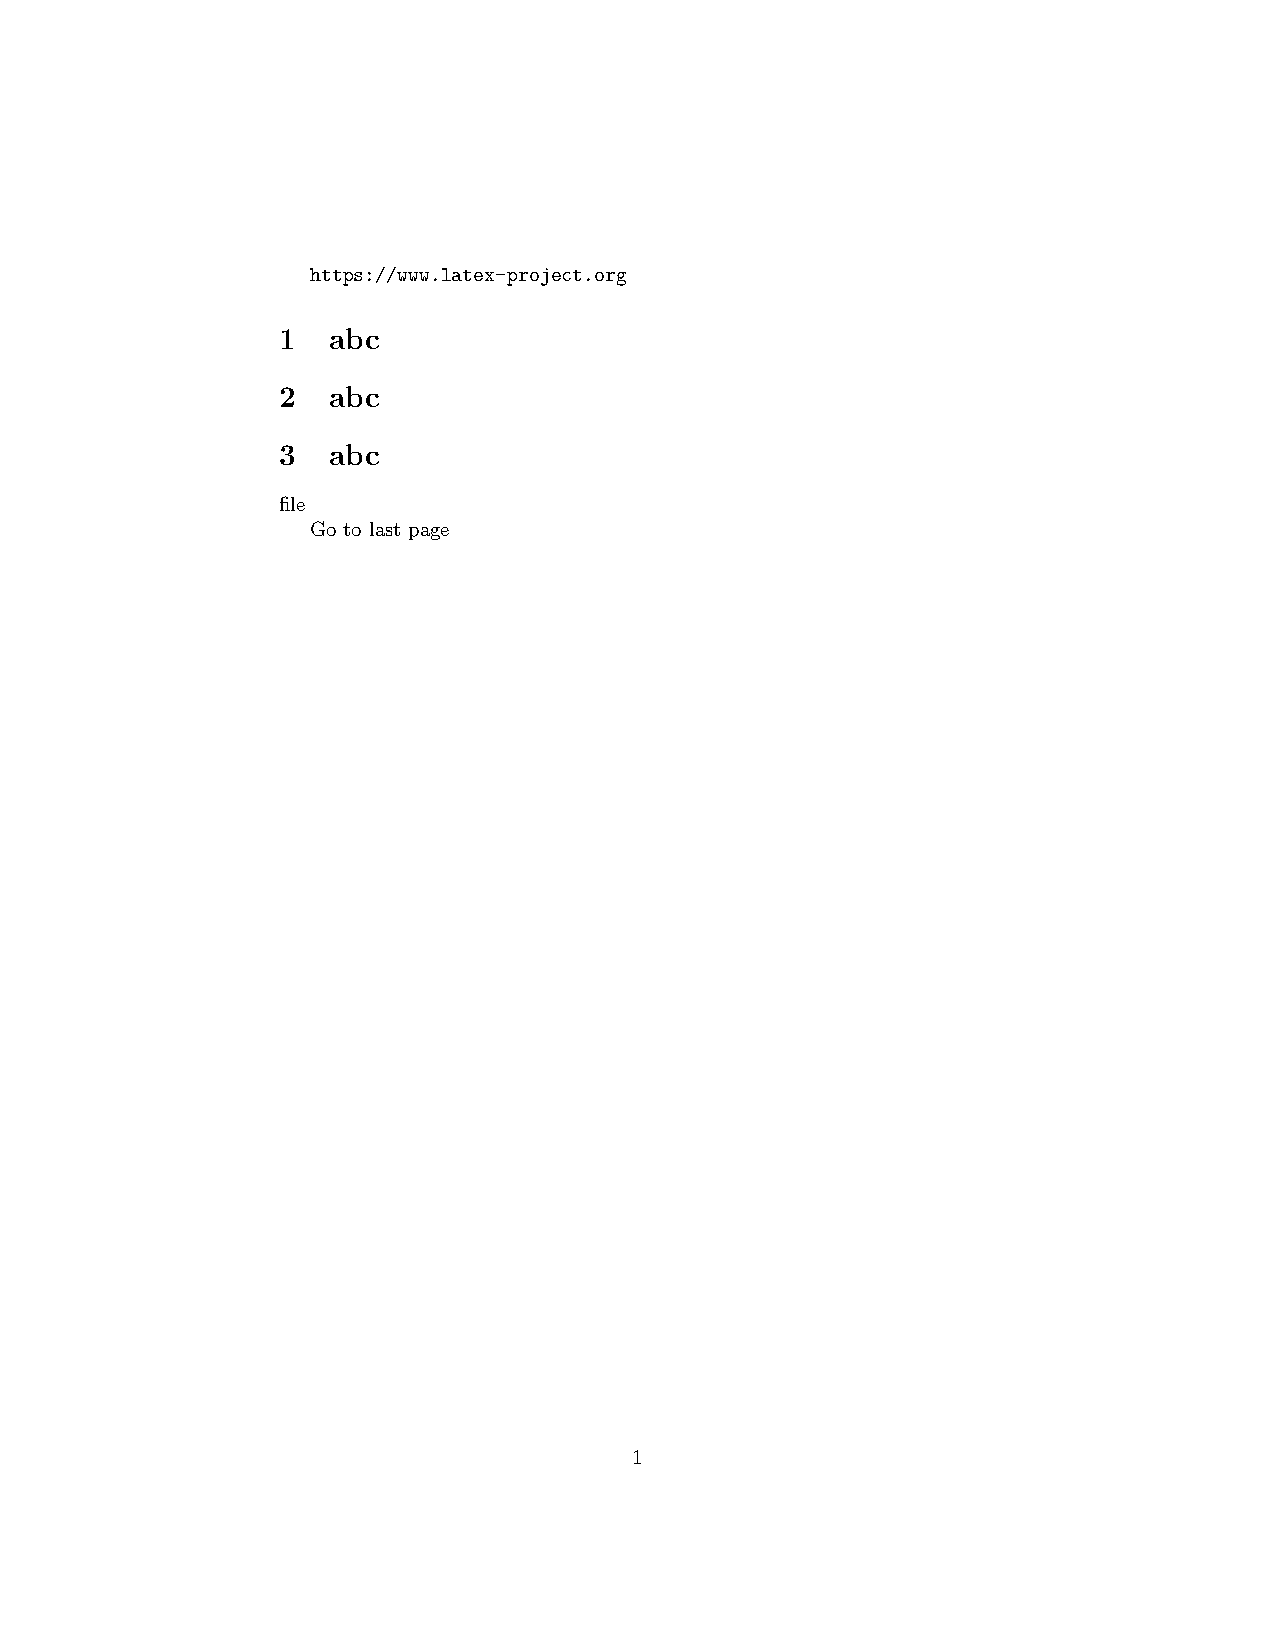
\includepdf[pages=-]{figure/pax-input2}
\end{document}
